\documentclass[12pt]{article}
\usepackage{geometry}
\geometry{margin=1in}
\usepackage{graphicx}
\usepackage{hyperref}
\usepackage{tikz}
\usepackage{tikz-3dplot}
\usepackage{pgfplots}
\usepackage{pgfplotstable}
\usepackage{tabularx}
\usepackage{amsmath, amssymb}

\title{Engineering Report --- Laurel Height Secondary School 
Electric Vehicle Club}
\author{Ayden Chiu}
\date{\today}

\begin{document}

\maketitle

\begin{abstract}
After the cancelation of 24V race, the motor that LHSS
EVC owns no longer fits our purpose of 12V race. A new drivetrain configuration
, steering system, and vehicle chasis has to be created in order to maximize, 
speed, efficiency, and minimize weight for 805. 
Two Kraken X60 motors and a gearbox providing 12:1 ratio
was purchased. By testing the vehicle on track, data shows positive results,
generating a speed of up to 40 km/h, and having 
sufficient capacity to finish the race. Therefore, 
the new vehicle 805 is believed to succeed in our next race with the new design.
\end{abstract}

\section{Introduction}

\subsection{Project Overview}
The race vehicle, 803's performance in the Waterloo EV Challenge October race 2025
was not optimal. Although the vehicle leads the race 
in the first 15 minutes, the battery capacity deteriates 
rapidly, leading to the inability to finish the race.

\subsection{Problem Statement}
803 was equipped with one Saietta BR-119-R-68 motor,
designed for 48V use. According to the technical specification
provided by the manufacturer, the motor can create a torque of 12.1 Nm.
Yet, due to the nature of 48V motor, it lacks the ability to 
provide efficient run in 12V useage. The motor consumes 
amperage over our expectation, and therefore leading to our
early end in the race. Additionally, the motor weighs 11kg,
increasing the weight of the car, therefore requires more
energy to accelerate. Moreover, the vehicle is equipped with
anti-ackermann steering system, which does not benefit our
relatively low-speed race.  

\subsection{Design Objectives}
After analysis from the preivous race, the following goals are created
\begin{enumerate}
  \item To create new steering system that allows efficient turns
  \item To increase the vehicle top speed to above 35 km/h
  \item To increase the efficiency of drivetrain, and successfully finish the race (70 minutes)
  \item To reduce weight of the vehicle
\end{enumerate}


\section{Background}

\subsection{Competition Overview}
The competition occurs at the parking lot area around the 
East Campus of University of Waterloo. The race track is
around 950m, with 4 major turns (Figure 1.1). 

\begin{figure}[htbp]
  \centering
  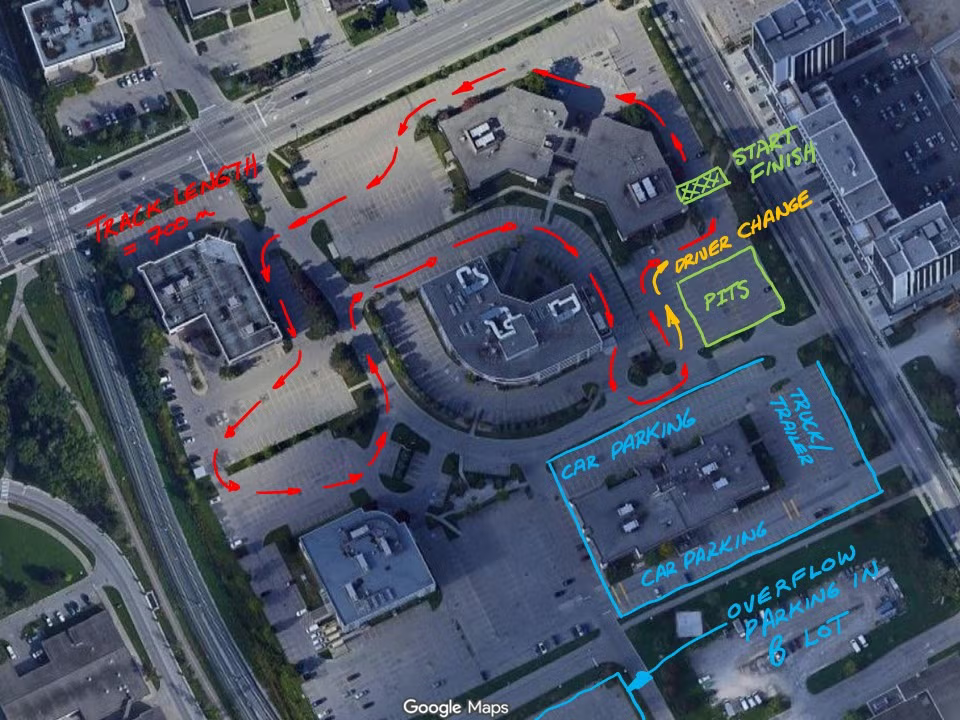
\includegraphics[width=0.7\textwidth]{Course.png} 
  \caption{Course for May 2026 Race}
\end{figure}

\newpage

\subsection{Design Constraints}
Rules for 2026 Races are as follows,  
\begin{enumerate}
  \item Distance between tires must be at least 0.90 m
  \item Vehicle no wider than 1.2m
  \item Maximum vehicle length is 3.5m
  \item Driver must be in a seated, forward-facing position
  \item Frame must has sufficient strucutal strength to protect the Driver
  \item Two horizontal member spaced 6 to 10 inches apart to protect driver's legs
  \item Steel / Aluminum
  \item Roll bar must extend at least 50mm over the top of the helmet
  \item The steering must allow for a turn within a radius of 5m
  \item MTX-35 battery only
  \item Battery must be secured
  \item Driver must of complete manual control of the vehicle
\end{enumerate}



\section{Methodology}

\subsection{Frame}

\subsubsection*{Materials}

The perivous vehicle generations used steel as frames. However, such design 
would increase the weight of the vehicle. Therefore, the current design now
accquires aluminum as the main material. 

According to simulation, the weight is reduced form 64.4 kg to 22.5 kg. This
significantly reduced the amount of energy needed to accelerate 805 to its top speed.

\newpage

\subsubsection*{Design}

805 shares the same frame with 804. The design seperate 805 into three sections: 
Leg, Body, Back.

\begin{figure}[htbp]
  \centering
  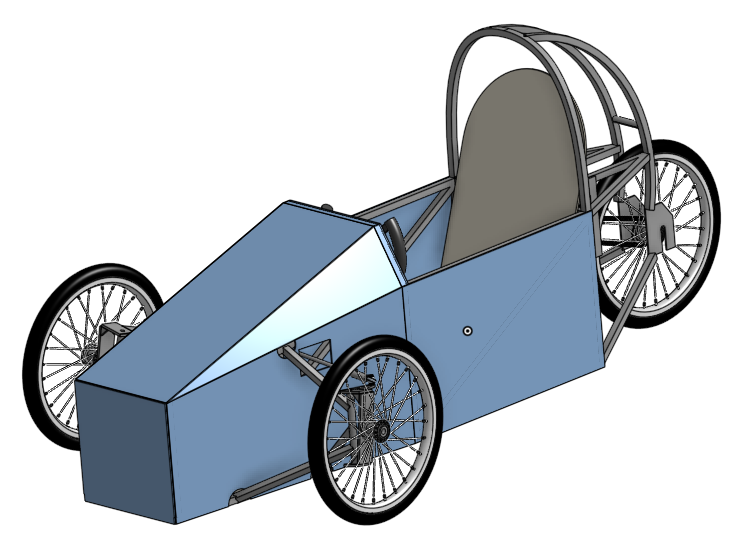
\includegraphics[width=0.7\textwidth]{Car.png} % or figures/myphoto.png
  \caption{805 Design.}
\end{figure}

The leg section is the front portion of 805. It provides room for driver's leg,
steering systems, and a MTX-35 battery. 

The battery is located at the most front of the car. This location allows for a
more balanced weight distribusion across the car, counteracting the center of mass
of the driver. The battery is held secure by the battery holder. This holder set contains
two rods that bolds the battery at its position, with four-sided barriers at the bottom,
preventing the battery from leaving its position.

\begin{figure}[htbp]
  \centering
  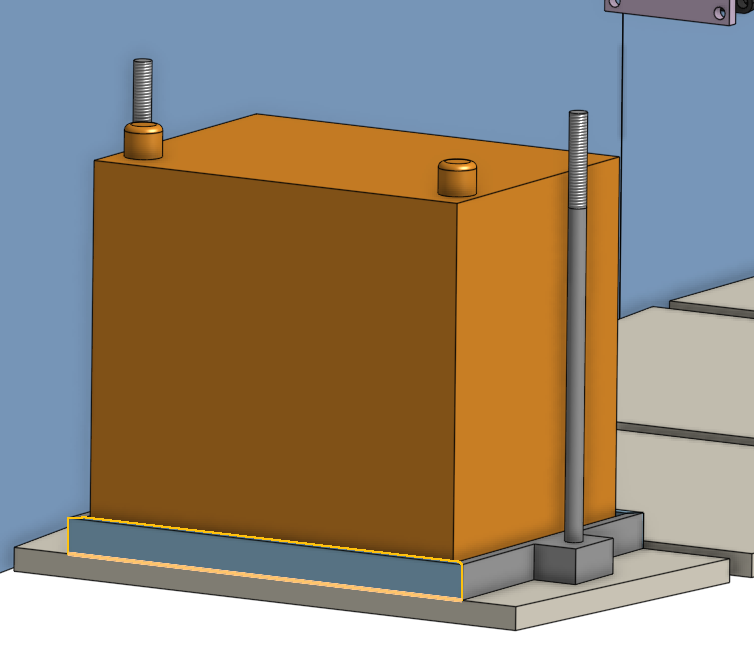
\includegraphics[width=0.3\textwidth]{Battery.png} % or figures/myphoto.png
  \caption{Battery Design.}
\end{figure}

A footrest is created in preventing the driver from knocking off the battery from
the fixed location.

\begin{figure}[htbp]
  \centering
  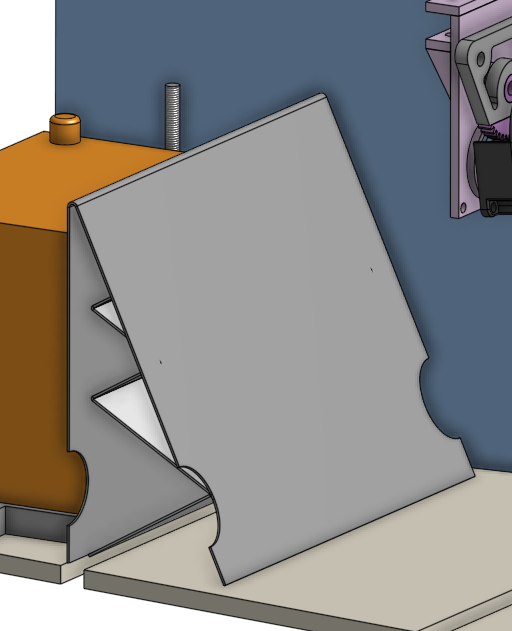
\includegraphics[width=0.3\textwidth]{footstep.png} % or figures/myphoto.png
  \caption{Footrest Design.}
\end{figure}

The steering gearbox is located at the middle-top crossbar, bolted in place. The
specific details of this gearbox will be discussed in section 3.2.

\begin{figure}[htbp]
  \centering
  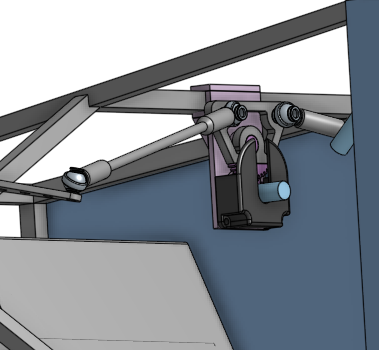
\includegraphics[width=0.4\textwidth]{steeringLoc.png} % or figures/myphoto.png
  \caption{Steering Location Design.}
\end{figure}

The leg section is covered by three panels (top, left, and right). The design
of these three panels is to streamline the vehicle, therefore reducing the drag
coefficient. 

\begin{figure}[htbp]
  \centering
  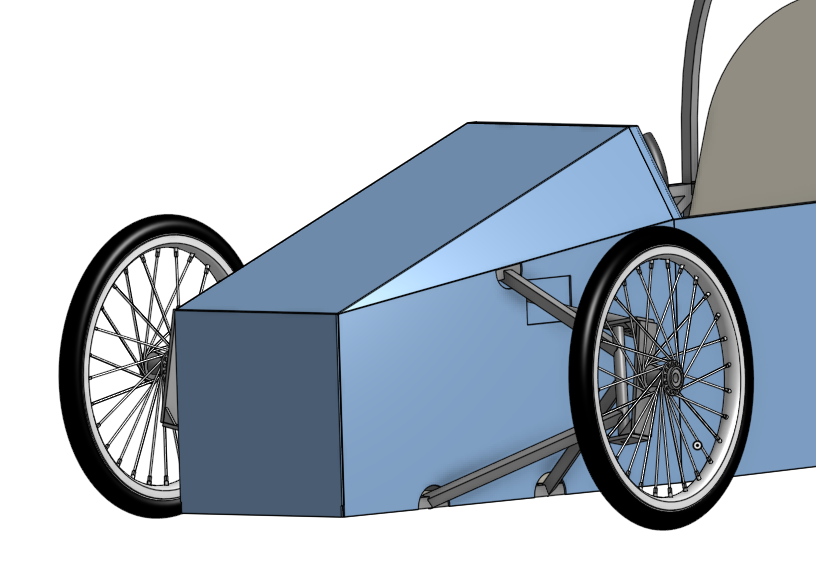
\includegraphics[width=0.4\textwidth]{leg.png} % or figures/myphoto.png
  \caption{Front Panel Design.}
\end{figure}

\newpage

The body section is where the driver sits and operates. This section contains the kill
switch (in yellow), yoke, and driver seat. 

The yoke is directly connected to three steering bar, with 2 universial joints in order
to control the steering gearbox. The driver sits on a wood plate, which provides an
incline that not only reduces the coefficient of drag, but to allow the driver to see a
minimum distance of 2 meters in front of the car. The kill switch is on the right side of
the driver, which provides easy access in case of an emergency.

\begin{figure}[htbp]
  \centering
  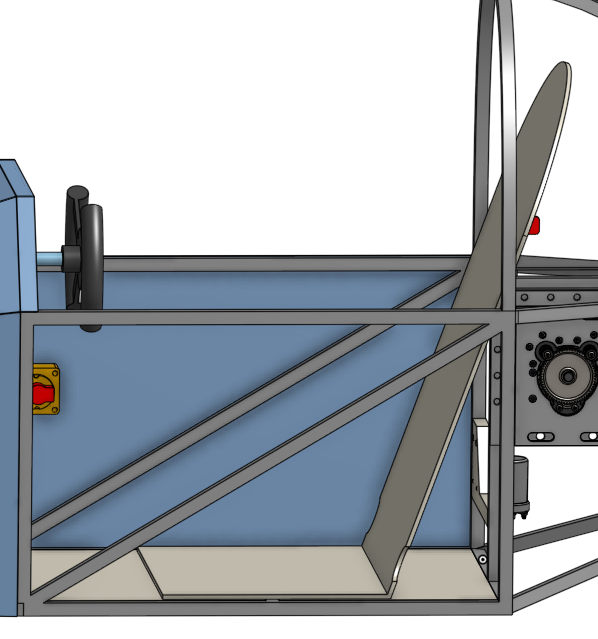
\includegraphics[width=0.4\textwidth]{body.png} % or figures/myphoto.png
  \caption{Body Section Design.}
\end{figure}

\newpage



%has to include all components, and potientially changing the picture after design
The back section of the car stores every compoenents of the drivetrain. Two Kraken X60s
are mounted to a flipped gearbox, and the gearbox is attached to two mountaing plates.
After a gear reduction of 9:1, the gearbox will then export the rotational energy to 
a sprocket that is connected to the rear wheel. 

The two motors are connected via wires, to a CANBUS and Rasberry Pi control unit. They are
stored and mounted on the panel located above the wheel. 

A roll-cage is designed to start from the bottom of 805, and bends over the driver's
helmet. A 50mm clearance is engaged in protection for the driver's safety. Two bent support
beam is connected from the top of the roll-cage to rear mount of the vehicle (Figure 8).

\begin{figure}[htbp]
  \centering
  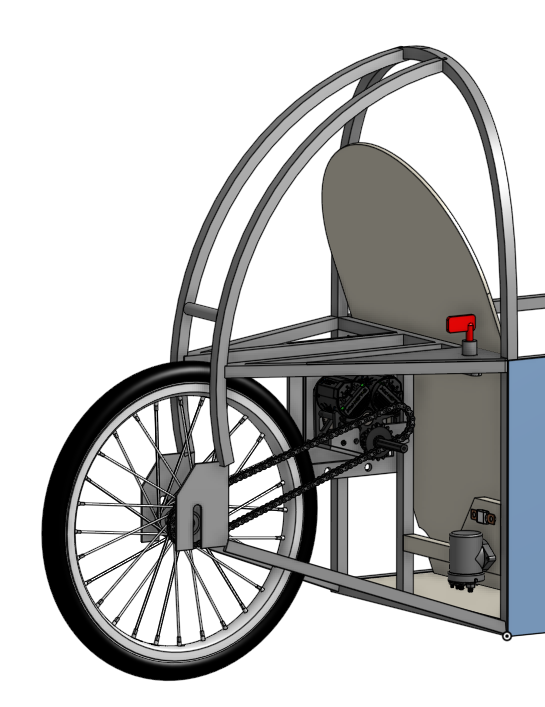
\includegraphics[width=0.4\textwidth]{back_section.png} % or figures/myphoto.png
  \caption{Back Section Design.}
\end{figure}

805 is equipped with 19-in diameter bicycle wheel, including the two forward wheel and rear wheel. This design provides significant amount
of torque transfer from motor to the ground. Furthermore, the design of bicycle wheel
reduces a significant amount of frictional force, allowing 805 to operate efficiently.


\subsection{Steering System}




\subsection{Drivetrain}

\subsubsection*{Overview}

Due to the unsatifactory results in October Race, the team has come to a conclusion that
804 lacks the efficiency and energy in order to finish the race. Therefore, a motor that
is designed for 12V race should be used on 805.

After researches, the design team has found a few suitable industrial motors that operates
at 12V. Yet, none of the motor manufacturer replied the message, and such path was stalled.

Robotics motor has become the only option for the team. Consulting with serval FIRST robotics 
team members at the club, the Kraken X60s shows the best and is considered as the optimal motor
for our situation. Other alternate motors include Kraken X44, NEO Vortex, NEO 2.0.

\subsubsection*{Performance Data}

From data aquired from online resources, the following graph is created in order to 
determine the operation RPM, torque, and current.

\begin{figure}[htbp]
  \centering
  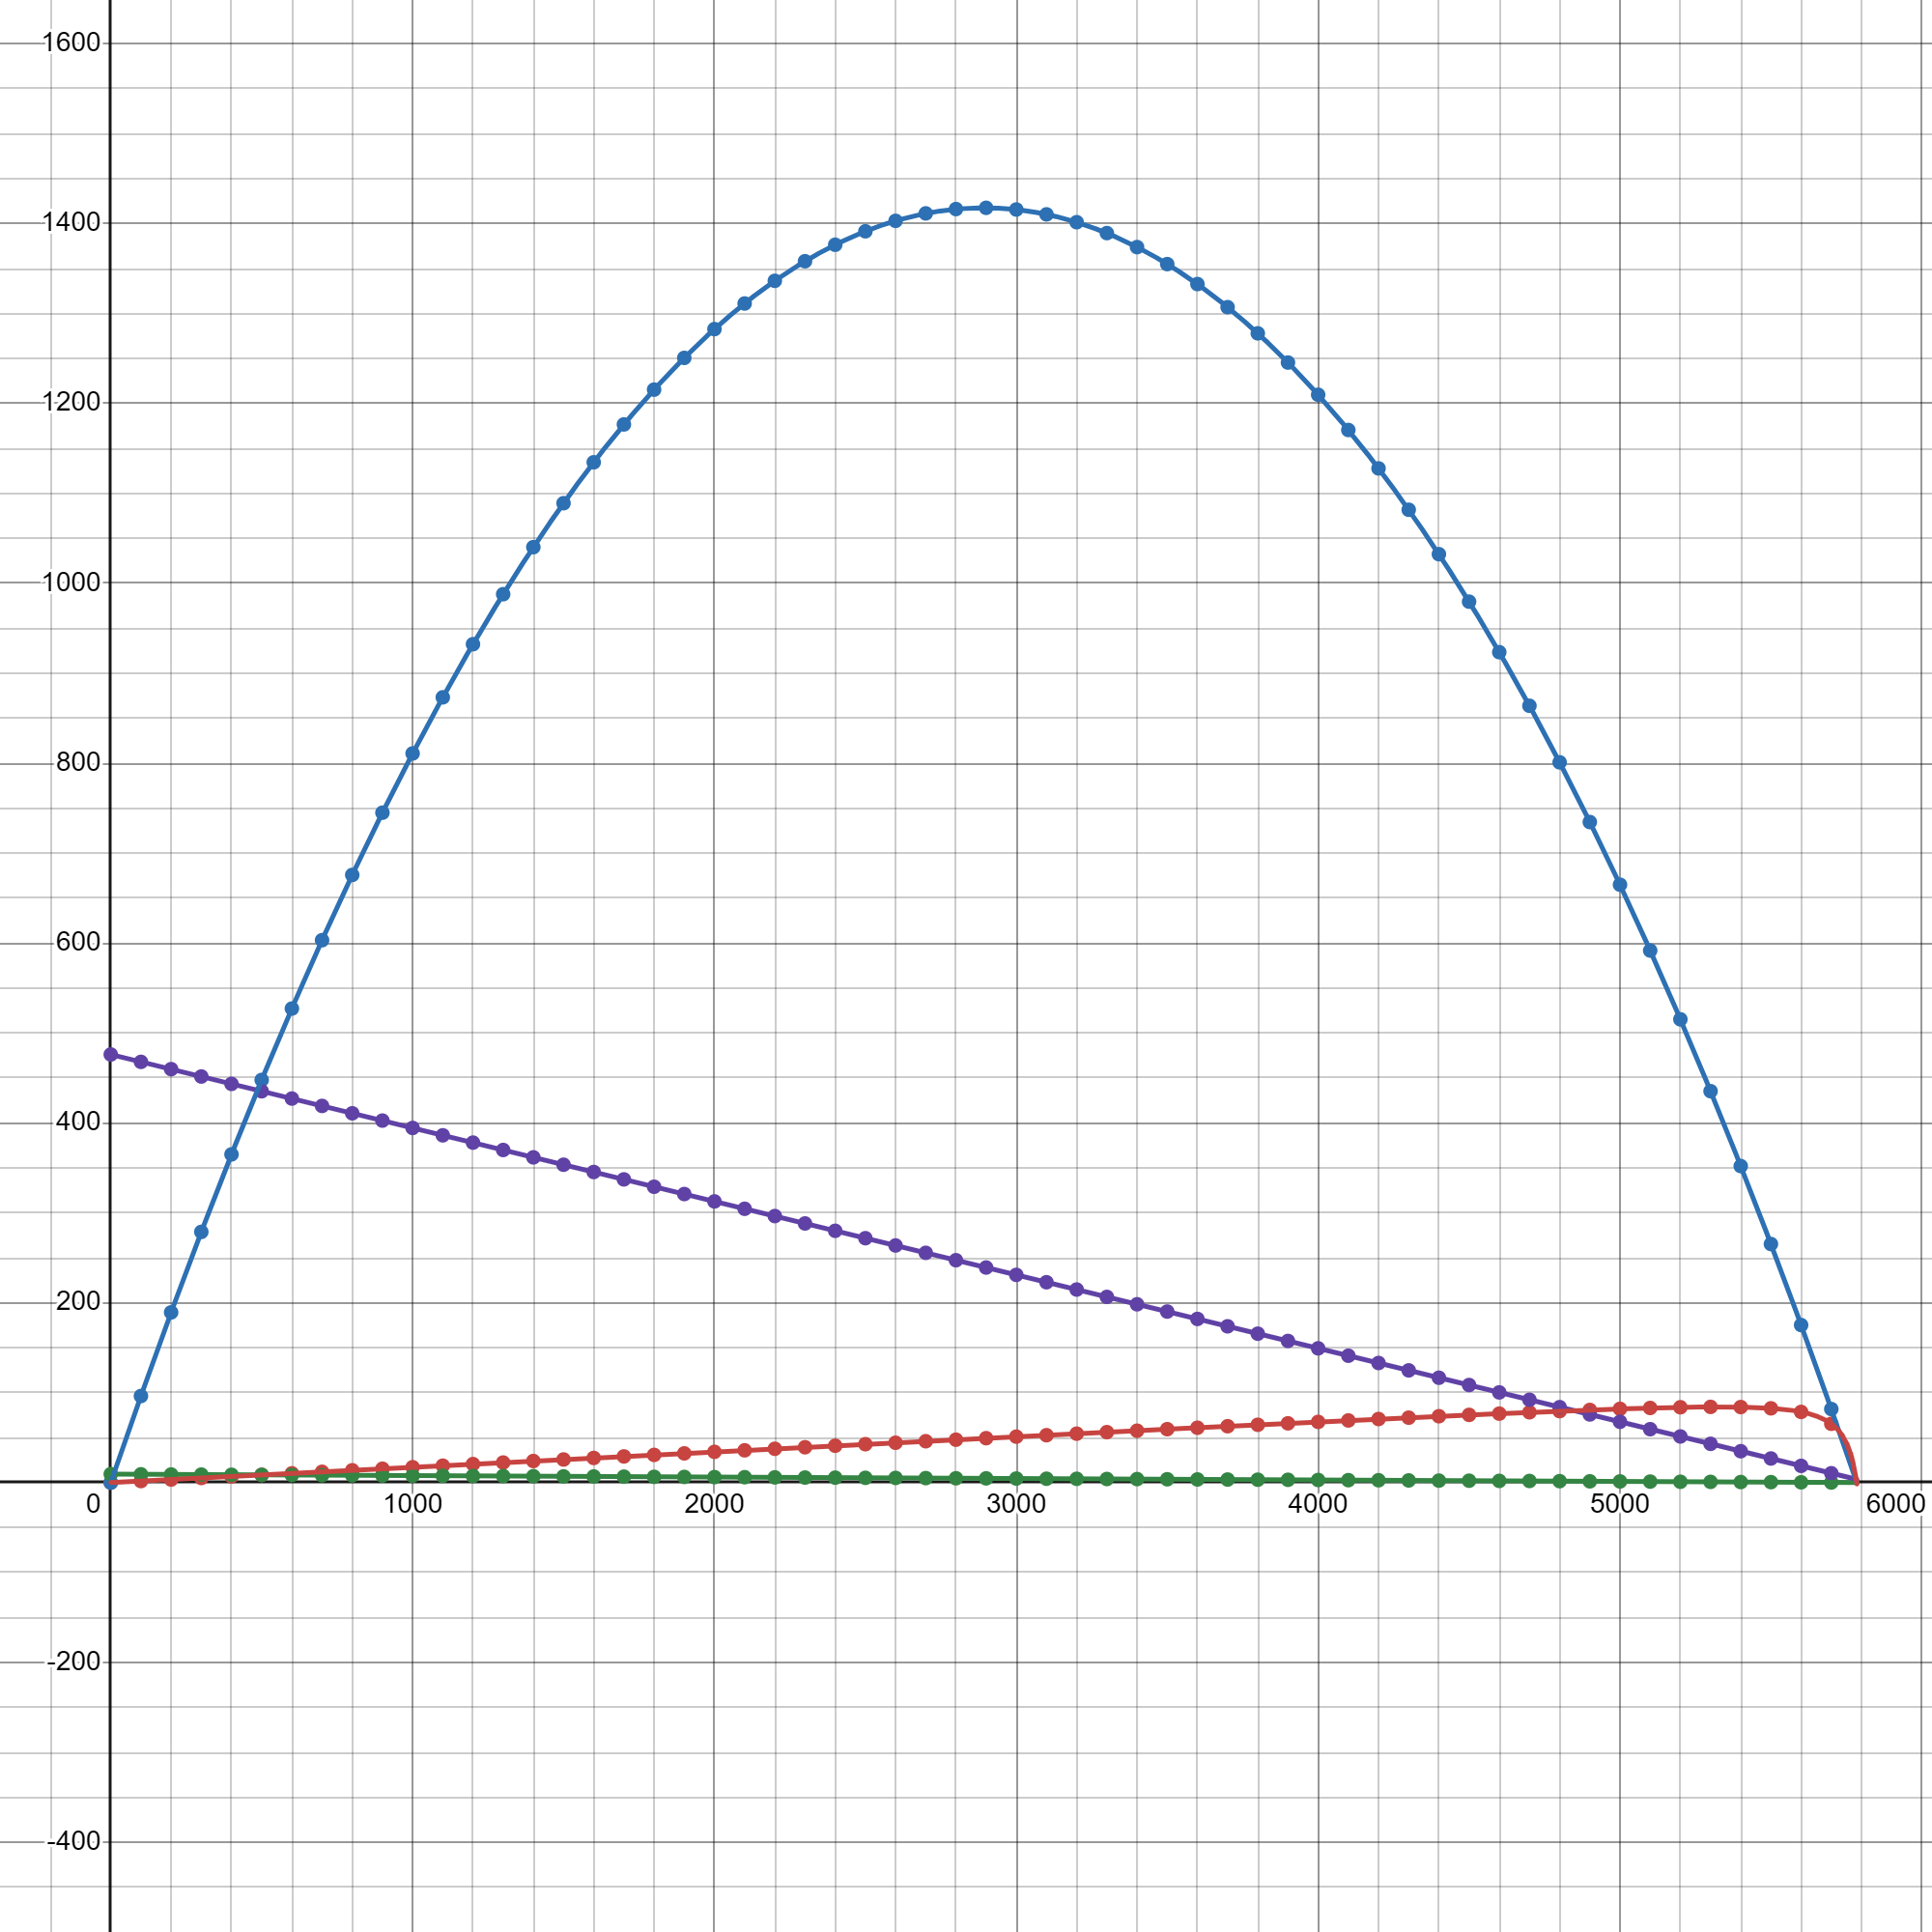
\includegraphics[width=0.6\textwidth]{Kraken X60.png} % or figures/myphoto.png
  \caption{Kraken X60 Performance.}
\end{figure}

The x-axis is the RPM value;
the blue line indicates the Power (W); the purple line indicates the current consumed (A);
the green line indicates the Torque (Nm); the red line indicates the Efficiency.

The following link describes the above graph:

\url{https://www.desmos.com/calculator/baupqlsyxa}

\newpage

\subsubsection*{Calculations: Maximum Current Delivers}

A prelimary calculation is needed to determine the maximum currrent that can be delievred
to the motor, in order to successfully finish the race. 

The 12V Race requires 805 to equip with a single MTX-35 battery. MTX-35 is regarded as
lead-acid battery. The following are specifications of MTX-35:

\begin{enumerate}
  \item Weight: 18.1 kg 
  \item Reserve Capacity@25 Amps: 100 minutes
  \item Voltage: 12V
  \item Capacity: 55Ah
  \item Maximum Amperage Intensity: 800 A
  \item AGM Battery (Lead-Acid)
\end{enumerate}

Instead of Watt's Law that governs the general battery performance, Lead-Acid battery are
more accurately represented through the Peukert's Law, which is as follows:
\begin{equation}
  C_p = I^k \times T
\end{equation}

\textbf{$C_p$}  is the capacity at a one-ampere discharge rate, which must
be expressed in ampere hours; $I$ is the actual discharge
current (i.e.current drawn from a load) in amperes; $t$ is the
actual time to discharge the battery, which must be expressed in hours; $k$
is the Peukert constant (dimensionless).


To find the Peukert's in the race situation, Equation 2 is used to determine the Peukert's constant (k).

\begin{equation}
  k = \frac{\log(t_2) - log(t_1)}{log(I_1) - log(I_2)}
\end{equation}


The two discharging values can be found through the 20-hour rate and RC rate. The
20-hour rate is the capacity listed (55Ah), where current is 2.75A by simple division.
Reserve Capacity shows the dischanging rate under high load, which is 1.67 hr at 25A.

Subsituting these into the equation,

\[k = \frac{\log(1.67)-\log(20)}{\log(2.75)-\log(25)}\]
\[k = 1.125\]

With Peukert Constant for MTX-35, we can use equation 1 to determine the maximum current
can be drawn continuously throughout the race. Assume the time is at 75 minutes (1.25), with 5
minutes of energy reserve. 

\[C_p = I^k \times T\]

The capacity can be expressed through the 20-hour rate, since the Peukert Capacity is unknown,

\[2.75^{1.125} \times 20 = I_{race}^{1.125} \times 1.25\]
\[I_{race} = 33.2 A\]

\[C_p = 2.75^{1.125} \times 20\]
\[C_p = 62.4 \text{Ah}\]

Therefore, 805 can only operate at a maximum current of 33.2 A continuously, with a
Peukert's capacity of 62.4 Ah.

\subsubsection*{Motor Performance At Maximum Current}

Since 805 is designed with two Kraken X60s connected in one flipped gearbox and has
a parallel connection, the current of the motor is halved to 16.6 A continuous.

From Figure 9's desmos graph, one Kraken X60's performance at 16.6 A is as below:
\begin{enumerate}
  \item Power: 158.8W
  \item Efficiency: 76.7\%
  \item RPM: 5624 RPM
  \item Torque: 0.258 Nm
\end{enumerate}

As a parallel-connected motor system, the following is the final performance from the two motors:
\begin{enumerate}
  \item Power: 317.6W
  \item Efficiency: 76.7\%
  \item RPM: 5624 RPM
  \item Torque: 0.516 NM
\end{enumerate}

The gearbox purchased has a gear ratio of $9:1$, which is further conencted a chain system of 24:18.
The final gear ratio is 12:1.

According to the Inverse Law between Torque and Speed,
\begin{equation}
  \frac{\tau_{input}}{\tau_{output}} = \frac{\text{Gear input}}{\text{Gear output}}
\end{equation}
\[\frac{0.516}{\tau_{output}} = \frac{1}{12}\]
\[\tau_{output} = 6.192 \text{~Nm}\]

\begin{equation}
  \frac{RPM_{input}}{RPM_{output}} = \frac{\text{Gear output}}{\text{Gear input}}
\end{equation}

\[\frac{5624}{RPM_{output}} = \frac{12}{1}\]
\[RPM_{output} = 468.7\]

Therefore, the wheel has an output speed of 468.7 RPM, with 6.192 Nm.


\subsubsection*{Stages of Race}

The race next operates with a constant speed. Turns and straights would affect
the current drawn from the battery. Therefore, 805 has to futher consider
the current drawn from the following three situations:
\begin{enumerate}
  \item Cruise
  \item Acceleration: 0-40 km/h
  \item Acceleration: 27-40 km/h
\end{enumerate}

Amperage drawn to maintain a top speed of 40 km/h is determiend through a simple $F_net$
statement:

\begin{equation}
  F_{net} = F_A - F_f - F_{AR}
\end{equation}


\bigskip


$F_{net}$ is derrived from Newton's Second Law, $F_{net} = ma$;

$F_A$ is the acceleration force provided by the Kraken motor;

$F_f$ is the frictional force against acceleration force;

$F_{AR}$ is the air resistance force agains acceleration force.

\subsubsection*{Cruise}

At cruise,

\[ 0 = F_A - \mu mg - \frac{1}{2}\rho v^2 C_D A \]
\[ F_A = \mu mg + \frac{1}{2}\rho v^2 C_D A \]

The following assumption and calculations are used:
\begin{itemize}
  \item $\mu$ (coefficient of friction) is 0.005, a typical rating of bike wheel running on asphalt;
  \item m (mass) is 116.5 kg;
  \item $\rho$ (air density) is 1.225;
  \item $v$ (velocity) is 11.11 m/s;
  \item $C_D$ (coefficient of drag) is 0.35;
  \item $A$ (front cross-sectional area) is 0.42;
\end{itemize}

\[ F_A = (0.005)(116.5)(9.81) + \frac{1}{2}(1.225)(11.11)^2(0.35)(0.42)\]
\[ F_A = 16.8 ~N\]

The acceleration force is 16.8 N.

With the acceleration force,
\[F_A = \frac{\tau}{r_{wheel}}\]
\[16.8 = \frac{\tau}{0.2413}\]
\[\tau = 4.054 \text{~Nm}\]

After gear ratio conversion, the torque from each individual motor is $0.169$ Nm. Refering
back to the motor performance graph, 
\begin{itemize}
  \item Power: 101.3 W
  \item Efficiency: 69.76\%
  \item Current: 12.1 A
  \item RPM: 5680 RPM\@ 
\end{itemize}

\subsubsection*{Accleration: 0-40 km/h}

This stage would only be used during start or driver change, therefore used three times only. 
805 is requried to stop fully and accelerate to its top speed.



\subsection{Utilizing the Phoenix6 API}

	In order to control the two Kraken X60 motors, the Phoenix6 software framework by CTR electronics is used in order to interface with the built-in TalonFX motor controllers in each motor repectively. The RoboRio, which is a FRC specific robotics controller was not chosen due to its cost. Instead, a Raspberry Pi 4b was opted to run the Phoenix6 software framework.

The following is a diagram of the architechture of the entire drivetrain:

\begin{figure}[htbp]
  \centering
  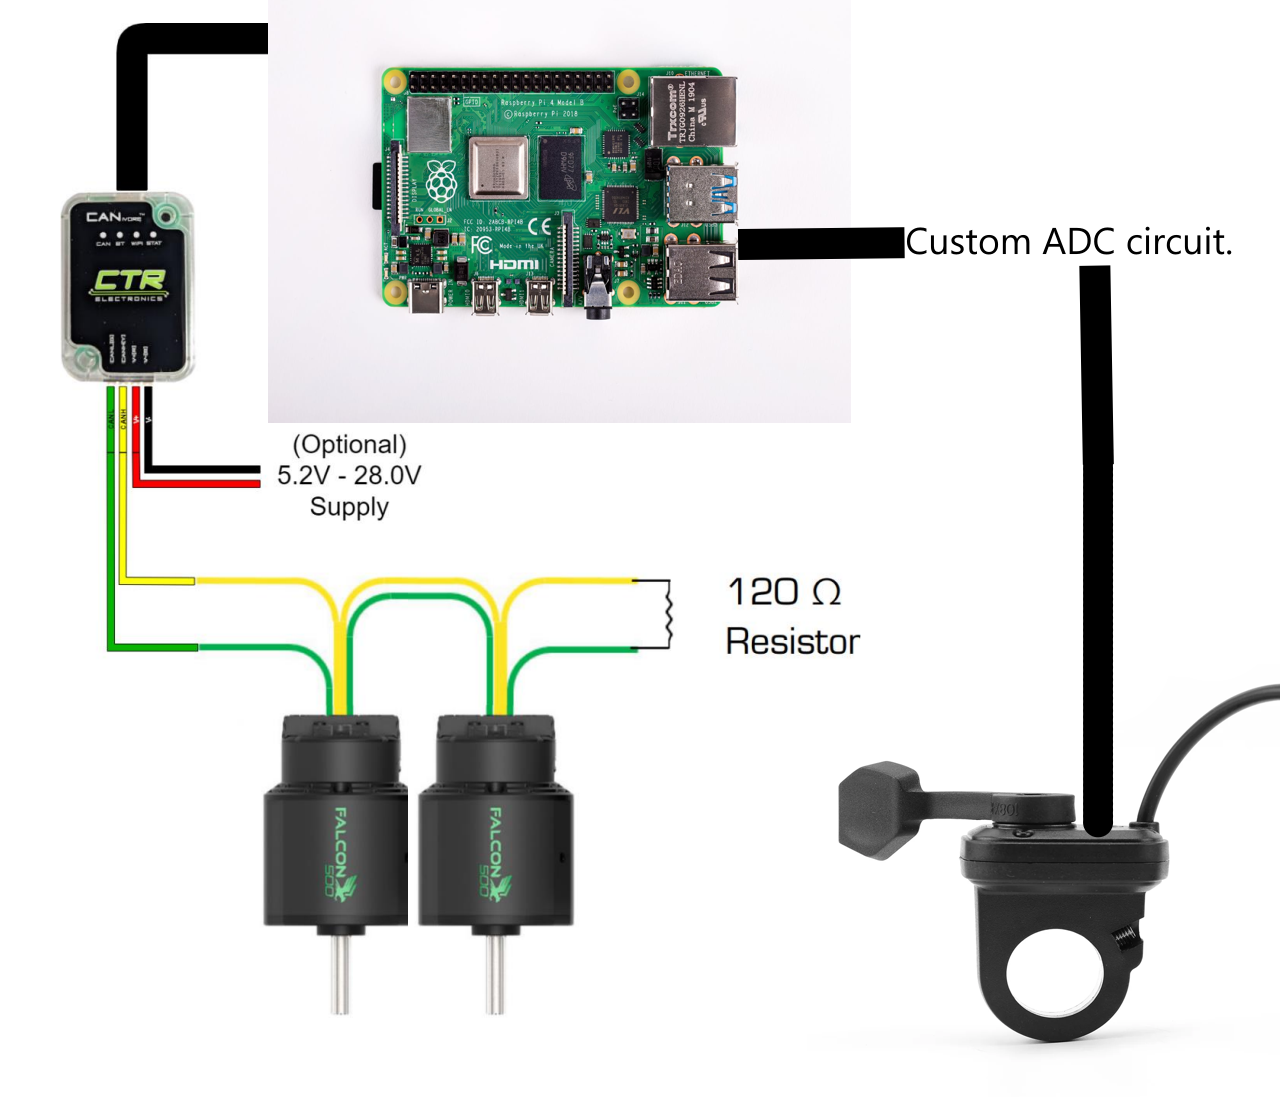
\includegraphics[width=0.4\textwidth]{DrivetrainArchitecture.png} % or figures/myphoto.png
  \caption{Electric Drivetrain Architechture.}
\end{figure}


Included are the following components:
\begin{enumerate}
	\item Throttle: Used as input to allow the driver to control the power fed to the motors.
	\item Analog to Digital converter: A custom built circuit to take in the 0.8 to 4.2 volt signal range and output UART serial data to be fed into the Raspberry PI.
	\item Raspberry Pi 4b: Handles processing of throttle data and sends CAN frames via CANBUS in order to control the motor.
 	\item Canivore: A USB to CAN adapter made by CTR Electronics.
	\item Kraken X60: Two motors in tandem used to power the rear wheel of the car.
\end{enumerate}


\subsection{Strategy}



\section{Results}
% Results content.

\section{Discussion}
% Discussion content.

\section{Conclusion}
% Conclusion content.

\bibliographystyle{plain}
\bibliography{references}

\end{document}
